\documentclass[tikz,border=2pt]{standalone}
\usepackage[T1]{fontenc}\usepackage{helvet}\usepackage{amsmath}
% shared TikZ styles for the three block diagrams (editable sources)
\usetikzlibrary{arrows.meta,positioning,fit,calc,backgrounds,shapes.geometric}
\definecolor{learn}{HTML}{6250D6}   % learned components
\definecolor{numer}{HTML}{2A78D6}   % numerical methods (Kalman lineage)
\definecolor{numerh}{HTML}{EB6834}  % numerical methods (Khalil lineage)
\definecolor{check}{HTML}{1D6B43}   % deterministic checks
\definecolor{ink}{HTML}{1B2430}
\definecolor{mut}{HTML}{5D6B7A}
\tikzset{
  every node/.style={font=\sffamily\scriptsize,text=ink,execute at begin node={\hyphenpenalty=10000 \exhyphenpenalty=10000 }},
  box/.style={draw=mut,rounded corners=1.5pt,line width=0.5pt,align=center,inner sep=3.5pt,fill=white,minimum height=6.5mm},
  learned/.style={box,draw=learn,dashed,line width=0.8pt,fill=learn!7},
  numeric/.style={box,draw=numer,line width=0.8pt,fill=numer!7},
  numerich/.style={box,draw=numerh,line width=0.8pt,fill=numerh!8},
  checkb/.style={box,draw=check,line width=0.8pt,double,double distance=0.6pt,fill=check!6},
  user/.style={box,fill=black!5},
  arr/.style={-{Stealth[length=4pt,width=3.4pt]},line width=0.5pt,draw=ink},
  darr/.style={arr,dashed},
  lab/.style={font=\sffamily\fontsize{6}{7}\selectfont,text=mut,align=center},
  onl/.style={lab,fill=white,inner sep=1.5pt},
  group/.style={draw=mut,dotted,line width=0.6pt,rounded corners=3pt,inner sep=5pt},
}

\tikzset{every node/.append style={font=\sffamily\footnotesize}, lab/.style={font=\sffamily\fontsize{7}{8}\selectfont,text=mut,align=center}, onl/.style={lab,fill=white,inner sep=1.5pt}}
\begin{document}
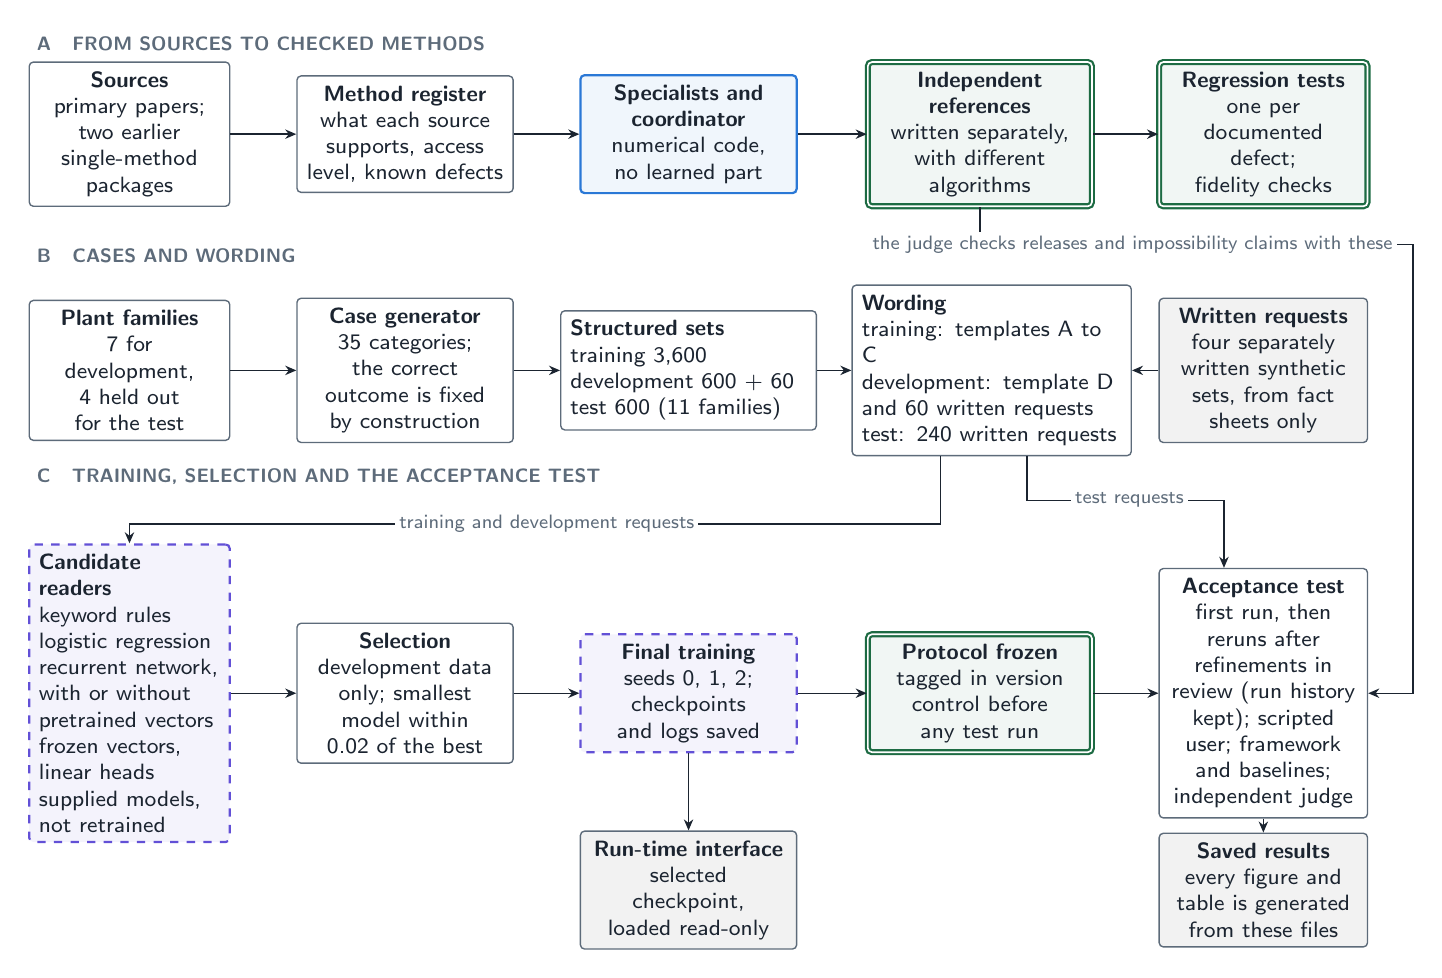
\begin{tikzpicture}[x=1cm,y=1cm]
% ---------------- row A: sources to methods ----------------
\node[lab,anchor=west] at (-1.3,8.45) {\textbf{A\quad FROM SOURCES TO CHECKED METHODS}};
\node[box,text width=2.3cm] (A1) at (0,7.3) {\textbf{Sources}\\ primary papers; two earlier single-method packages};
\node[box,text width=2.5cm] (A2) at (3.5,7.3) {\textbf{Method register}\\ what each source supports, access level, known defects};
\node[numeric,text width=2.5cm] (A3) at (7.1,7.3) {\textbf{Specialists and coordinator}\\ numerical code, no learned part};
\node[checkb,text width=2.6cm] (A4) at (10.8,7.3) {\textbf{Independent references}\\ written separately, with different algorithms};
\node[checkb,text width=2.4cm] (A5) at (14.4,7.3) {\textbf{Regression tests}\\ one per documented defect; fidelity checks};
\draw[arr] (A1) -- (A2); \draw[arr] (A2) -- (A3); \draw[arr] (A3) -- (A4); \draw[arr] (A4) -- (A5);
% ---------------- row B: data ----------------
\node[lab,anchor=west] at (-1.3,5.75) {\textbf{B\quad CASES AND WORDING}};
\node[box,text width=2.3cm] (B1) at (0,4.3) {\textbf{Plant families}\\ 7 for development, 4 held out for the test};
\node[box,text width=2.5cm] (B2) at (3.5,4.3) {\textbf{Case generator}\\ 35 categories; the correct outcome is fixed by construction};
\node[box,text width=3.0cm,align=left] (B3) at (7.1,4.3) {\textbf{Structured sets}\\ training 3,600\\ development 600 + 60\\ test 600 (11 families)};
\node[box,text width=3.3cm,align=left] (B4) at (10.95,4.3) {\textbf{Wording}\\ training: templates A to C\\ development: template D and 60 written requests\\ test: 240 written requests};
\node[box,fill=black!5,text width=2.4cm] (B5) at (14.4,4.3) {\textbf{Written requests}\\ four separately written synthetic sets, from fact sheets only};
\draw[arr] (B1) -- (B2); \draw[arr] (B2) -- (B3); \draw[arr] (B3) -- (B4); \draw[arr] (B5) -- (B4);
% ---------------- row C: training and selection ----------------
\node[lab,anchor=west] at (-1.3,2.95) {\textbf{C\quad TRAINING, SELECTION AND THE ACCEPTANCE TEST}};
\node[learned,text width=2.3cm,align=left] (C1) at (0,0.2) {\textbf{Candidate readers}\\ keyword rules\\ logistic regression\\ recurrent network, with or without pretrained vectors\\ frozen vectors, linear heads\\ supplied models, not retrained};
\node[box,text width=2.5cm] (C2) at (3.5,0.2) {\textbf{Selection}\\ development data only; smallest model within 0.02 of the best};
\node[learned,text width=2.5cm] (C3) at (7.1,0.2) {\textbf{Final training}\\ seeds 0, 1, 2; checkpoints and logs saved};
\node[checkb,text width=2.6cm] (C4) at (10.8,0.2) {\textbf{Protocol frozen}\\ tagged in version control before any test run};
\node[box,text width=2.4cm] (C5) at (14.4,0.2) {\textbf{Acceptance test}\\ first run, then reruns after refinements in review (run history kept); scripted user; framework and baselines; independent judge};
\draw[arr] (C1) -- (C2); \draw[arr] (C2) -- (C3); \draw[arr] (C3) -- (C4); \draw[arr] (C4) -- (C5);
% cross links
\draw[arr] (10.3,0 |- B4.south) -- (10.3,2.35) -| (C1.north);
\node[onl] at (5.3,2.35) {training and development requests};
\draw[arr] (11.4,0 |- B4.south) -- (11.4,2.65) -| ($(C5.north)+(-0.5,0)$);
\node[onl] at (12.7,2.65) {test requests};
\draw[arr] (A4.south) -- (A4.south |- 0,5.9) -- (16.3,5.9) |- (C5.east);
\node[onl,anchor=east] at (16.1,5.9) {the judge checks releases and impossibility claims with these};
% outputs
\node[box,fill=black!5,text width=2.4cm] (O1) at (14.4,-2.3) {\textbf{Saved results}\\ every figure and table is generated from these files};
\node[box,fill=black!5,text width=2.5cm] (O2) at (7.1,-2.3) {\textbf{Run-time interface}\\ selected checkpoint, loaded read-only};
\draw[arr] (C5) -- (O1); \draw[arr] (C3) -- (O2);
\end{tikzpicture}
\end{document}
